\pdfinfo{
    /Author (Luca Fantin, Matteo Zanella)
    /Title (Exact and heuristic approaches to the Travelling Salesman Problem (TSP))
    /Keyword (TSP, Heuristic, CPLEX)
}

% Libraries
\documentclass[a4paper,12pt]{report}
\usepackage[utf8]{inputenc}
\usepackage[english]{babel}
\usepackage{fancyhdr}
\usepackage{sectsty}
\usepackage[inner=3cm,top=2cm,bottom=2cm,outer=2cm]{geometry}
\usepackage{setspace}
\usepackage[hang,small,sf,font=small, labelfont=bf]{caption}
\usepackage{subcaption}
\usepackage[usenames]{color}
\usepackage{xcolor}
\usepackage{colortbl}
\usepackage{tocloft}
\usepackage[a-1b]{pdfx}
\usepackage{hyperref}
\usepackage{tabto}
\usepackage{mathtools}
\usepackage{bbold}
\usepackage{wrapfig}
\usepackage[]{mdframed}
\usepackage{amsmath}
\usepackage{amsthm}
\usepackage{amssymb}
\usepackage{cases}
\usepackage{indentfirst}
\usepackage{afterpage}
\usepackage{placeins}
\usepackage{csquotes}

%images
\usepackage{graphicx}
\graphicspath{ {./images/} }

%tikz
\usepackage{tikz}
\usetikzlibrary{arrows.meta}

%pseudocode
\usepackage{algorithm}
\usepackage{algpseudocode}

\DeclarePairedDelimiter\floor{\lfloor}{\rfloor}
\DeclarePairedDelimiter\ceil{\lceil}{\rceil}
\setlength{\arrayrulewidth}{1pt}
\newcommand\blankpage{%
    \null
    \thispagestyle{empty}%
    \addtocounter{page}{-1}%
    \newpage}

% Mandatory settings
\onehalfspacing
\hypersetup{
    colorlinks,
    citecolor=black,
    filecolor=black,
    linkcolor=black,
    urlcolor=black
}

% Subsections
\renewcommand{\cftpartleader}{\cftdotfill{\cftdotsep}} % for parts
\renewcommand{\cftchapleader}{\cftdotfill{\cftdotsep}} % for chapters
\renewcommand{\cftsecleader}{\cftdotfill{\cftdotsep}} % for sections

\algnewcommand\algorithmicforeach{\textbf{for each}}
\algdef{S}[FOR]{ForEach}[1]{\algorithmicforeach\ #1\ \algorithmicdo}


\usepackage[sorting=none]{biblatex}

\addbibresource{bibl.bib}
% Start document
\begin{document}





\begin{titlepage}
\begin{center}


\includegraphics[height=0.13\textheight]{logo_unipd.png}
\hfill

\includegraphics[height=0.13\textheight]{logo_dei.png}
\newline
\newline

\vspace{0.8cm}
\textsc{\LARGE Universit\`{a} degli Studi di Padova}\\
\vspace{1.6cm}
\textsc{\large 	School of Engineering Department of Information Engineering}\\
\vspace{0.4cm}

\textsc{\large Master Degree in Computer Engineering}\\
\vfill
{ \LARGE \bfseries Exact and heuristic approaches to the Travelling Salesman Problem (TSP)}\\
\vspace{1cm}

\textbf{\large Operations Research 2}\\
\vfill

\raggedright\textbf{\large Supervisor:} \\
\raggedright\large Matteo Fischetti\\
\vfill
\raggedright\textbf{\large Candidates:} \\
\raggedright\large Luca Fantin (2119287)  \\
\raggedright\large Matteo Zanella (2122187)\\

\vfill
\centering{Academic Year 2023/2024}

\end{center}
\end{titlepage}

%\pagenumbering{roman}
%\thispagestyle{empty}
%\clearpage{\pagestyle{plain}\cleardoublepage}
    
%\clearpage\null\newpage

% Abstract
%\newcommand\summaryname{Abstract}
%\newenvironment{Abstract} {
%    \begin{center}%
%    \bfseries{\summaryname} \end{center}
%}
    
%\begin{Abstract}
%This is an example of an abstract.
%\end{Abstract}

% Index
\clearpage{\pagestyle{plain}\cleardoublepage}
\tableofcontents
%\listoffigures
%\listoftables

\clearpage{\pagestyle{plain}\cleardoublepage}
\pagenumbering{arabic}

%\afterpage{\blankpage}

% Introduction
\clearpage{\pagestyle{plain}\cleardoublepage}
\chapter{Introduction}

The \textit{Travelling Salesman Problem}, also known as \textit{\textbf{TSP}}, is one of the most famous and studied optimization problems in the Computer Science and Operations Research fields.\\
Although its first mathematical formulation was proposed in the 19th century by the mathematicians \textbf{William Rowan Hamilton} and \textbf{Thomas Kirkman}, it received scientific attention from the 1950s onwards.\\
In 1972, \textbf{Richard M. Karp} proved the \textbf{NP-hard nature} of the TSP; this meant that the computation time for any solving algorithm can grow exponentially with the input size. Despite this, many different approaches have been developed over the years, yielding both exact and approximate solutions.\\

In this paper, several algorithms are explained, developed and tested against each other, both exact and approximate.

\phantomsection
\addcontentsline{toc}{subsection}{Problem formulation}
\subsection*{Problem formulation}\label{Problem formulation}

In this thesis, we will consider an \textbf{undirected graph} $G=(V, E)$, where $V$ is a set of $|V|=N$ \textit{nodes} (or \textit{vertices}) and $E$ is a set of $|E|=M$ \textit{edges}.\\
We define a \textbf{Hamiltonian cycle} of $G$, $G^*=(V, E^*)$, as a graph whose edges form a cycle going through each node $v\in V$ exactly once.\\
We also define a \textbf{cost function} for the edges $c : E \rightarrow \mathbb{R}^+$, $c_e\coloneq c(e) \ \forall \ e\in E$.\\

The target of the TSP is finding an Hamiltonian cycle of G of minimum total cost, obtained by summing the costs of all edges in the cycle.\\
We can formulate this problem through \textit{Integer Linear Programming (ILP)}. First, we define the following decision variables to represent whether or not a certain edge is included in the Hamiltonian cycle:
$$x_e = \begin{cases}
  1 & \mbox{if } e\in E^*\\
  0 & \mbox{otherwise} \\
\end{cases} \qquad \forall \ e\in E$$
The ILP model is the following:
\begin{numcases}
  \displaystyle \min\,\sum_{e\in E}c_ex_e\\
  \displaystyle \sum_{e\in\delta(h)} x_e = 2 \quad \forall \ h\in V\label{HamiltCyc}
  \\
  \displaystyle \sum_{e\in\delta(S)} x_e\leq |S|-1 \quad \forall \ S\subset V : v_1 \in S\label{SEC}
  \\
  \displaystyle 0\leq x_e\leq1 \quad\mbox{integer} \quad \forall \ e\in E
\end{numcases}\\
Constraints \ref{HamiltCyc} impose that every node of the graph must be touched by exactly two edges of the cycle. This group of contraints alone isn't enough to guarantee to find a valid Hamiltonian Cycle: we could find lots of isolated cycles.\\
Constraints \ref{SEC}, called \textbf{Subtour Elimination Constraints (SEC)}, guarantee that any solution found through this model is made up of only one connected component: every vertex $v\neq v_1$ must be reachable from $v_1$.\\
Despite their importance, their number is exponential in $N$, thus, considering all of them at once is computationally expensive.


% Setup
\clearpage{\pagestyle{plain}\cleardoublepage}
\chapter{Project Setup}
...
\section{Performance profiler}
...

% Heuristics
\clearpage{\pagestyle{plain}\cleardoublepage}
\chapter{Heuristics}
A heuristic is any approach to problem solving that employs a practical method that is not fully optimized but it is sufficient to reach an immediate short-term goal or approximation.

Given the NP-Hard nature of the Travelling Salesman Problem, finding the optimal solution may require a long time, hence the need to have heuristics method to find solutions that are close to the optimal.

\section{Nearest Neighbor (Greedy)}

A first approach to the TSP is to iteratively build a solution by starting from a certain node and considering the edges with the smallest weights first when choosing the next node in the cycle.

This type of logic is called \textit{greedy}: a greedy algorithm looks for the locally optimal choice at each stage.

\begin{center}
    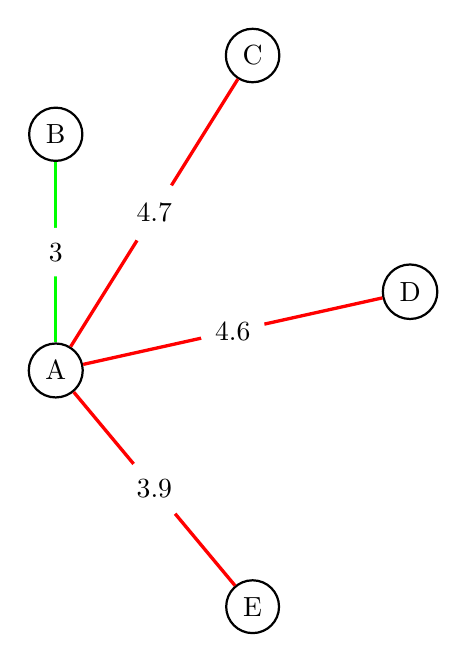
\begin{tikzpicture}
        \begin{scope}[every node/.style={circle,thick,draw}]
            \node (A) at (0,0) {A};
            \node (B) at (0,3) {B};
            \node (C) at (2.5,4) {C};
            \node (D) at (4.5,1) {D};
            \node (E) at (2.5,-3) {E};
        \end{scope}

        \begin{scope}[every node/.style={fill=white,circle},
                    every edge/.style={draw=red,very thick}]
            \path [-] (A) edge[draw=green] node {$3$} (B);
            \path [-] (A) edge node {$4.7$} (C);
            \path [-] (A) edge node {$4.6$} (D);
            \path [-] (A) edge node {$3.9$} (E);
        \end{scope}
    \end{tikzpicture}
\end{center}

In this example, among the edges connected to the node $A$, the edge $(A, B)$ is the one with the smallest weight, so node $B$ should be $A$'s successor.

By repeating this process for each new node added to the path and connecting the last node ($E$) to the starting node ($A$):

\begin{figure}[h]
    
    \centering
    \begin{subfigure}[c]{0.2\textwidth}
        \centering
        \resizebox{\linewidth}{!}{
            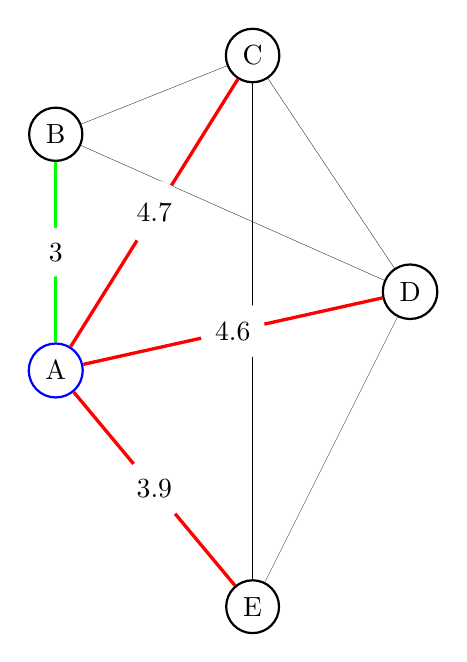
\begin{tikzpicture}
                \begin{scope}[every node/.style={circle,thick,draw}]
                    \node[draw=blue] (A) at (0,0) {A};
                    \node (B) at (0,3) {B};
                    \node (C) at (2.5,4) {C};
                    \node (D) at (4.5,1) {D};
                    \node (E) at (2.5,-3) {E};
                \end{scope}

                \begin{scope}[every node/.style={fill=white,circle},
                            every edge/.style={draw=red,very thick}]
                            \path [-] (B) edge[draw=black, ultra thin] (C);
                            \path [-] (B) edge[draw=black, ultra thin] (D);
                            \path [-] (C) edge[draw=black, ultra thin] (D);
                            \path [-] (C) edge[draw=black, ultra thin] (E);
                            \path [-] (D) edge[draw=black, ultra thin] (E);
                            \path [-] (A) edge[draw=green] node {$3$} (B);
                            \path [-] (A) edge node {$4.7$} (C);
                            \path [-] (A) edge node {$4.6$} (D);
                            \path [-] (A) edge node {$3.9$} (E);
                \end{scope}
            \end{tikzpicture}
        }
    \end{subfigure}$\Rightarrow$
    \begin{subfigure}[c]{0.2\textwidth}
        \centering
        \resizebox{\linewidth}{!}{
            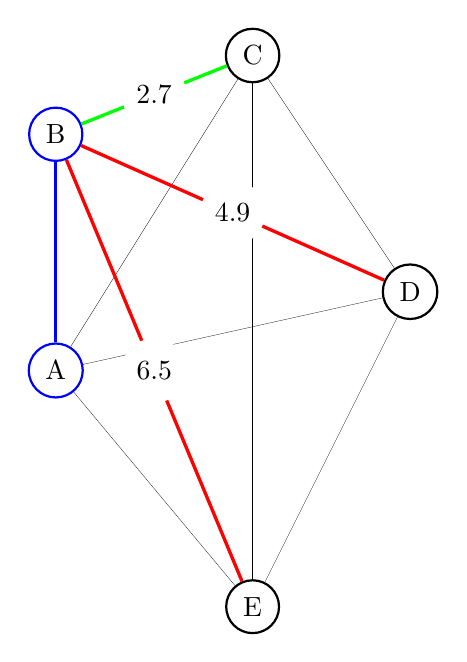
\begin{tikzpicture}
                \begin{scope}[every node/.style={circle,thick,draw}]
                    \node[draw=blue] (A) at (0,0) {A};
                    \node[draw=blue] (B) at (0,3) {B};
                    \node (C) at (2.5,4) {C};
                    \node (D) at (4.5,1) {D};
                    \node (E) at (2.5,-3) {E};
                \end{scope}

                \begin{scope}[every node/.style={fill=white,circle},
                            every edge/.style={draw=red,very thick}]
                    \path [-] (A) edge[draw=blue] (B);
                    \path [-] (C) edge[draw=black, ultra thin] (D);
                    \path [-] (D) edge[draw=black, ultra thin] (E);
                    \path [-] (E) edge[draw=black, ultra thin] (A);
                    \path [-] (A) edge[draw=black, ultra thin] (C);
                    \path [-] (A) edge[draw=black, ultra thin] (D);
                    \path [-] (C) edge[draw=black, ultra thin] (E);
                    \path [-] (B) edge[draw=green] node {$2.7$} (C);
                    \path [-] (B) edge[draw=red] node {$4.9$} (D);
                    \path [-] (B) edge[draw=red] node {$6.5$} (E);
                \end{scope}
            \end{tikzpicture}
        }
    \end{subfigure}$\Rightarrow$
    \begin{subfigure}[c]{0.2\textwidth}
        \centering
        \resizebox{\linewidth}{!}{
            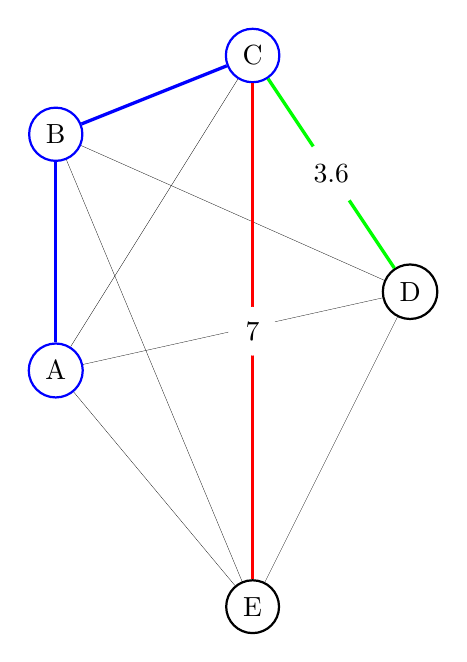
\begin{tikzpicture}
                \begin{scope}[every node/.style={circle,thick,draw}]
                    \node[draw=blue] (A) at (0,0) {A};
                    \node[draw=blue] (B) at (0,3) {B};
                    \node[draw=blue] (C) at (2.5,4) {C};
                    \node (D) at (4.5,1) {D};
                    \node (E) at (2.5,-3) {E};
                \end{scope}

                \begin{scope}[every node/.style={fill=white,circle},
                            every edge/.style={draw=red,very thick}]
                    \path [-] (A) edge[draw=blue] (B);
                    \path [-] (B) edge[draw=blue] (C);
                    \path [-] (C) edge[draw=green] node {$3.6$} (D);
                    \path [-] (D) edge[draw=black, ultra thin] (E);
                    \path [-] (E) edge[draw=black, ultra thin] (A);
                    \path [-] (A) edge[draw=black, ultra thin] (C);
                    \path [-] (A) edge[draw=black, ultra thin] (D);
                    \path [-] (B) edge[draw=black, ultra thin] (D);
                    \path [-] (B) edge[draw=black, ultra thin] (E);
                    \path [-] (C) edge[draw=red] node {$7$} (E);
                \end{scope}
            \end{tikzpicture}
        }
    \end{subfigure}$\Rightarrow$
    
\end{figure}
\begin{figure}[h]

    \centering$\Rightarrow$
    \begin{subfigure}[c]{0.2\textwidth}
        \centering
        \resizebox{\linewidth}{!}{
            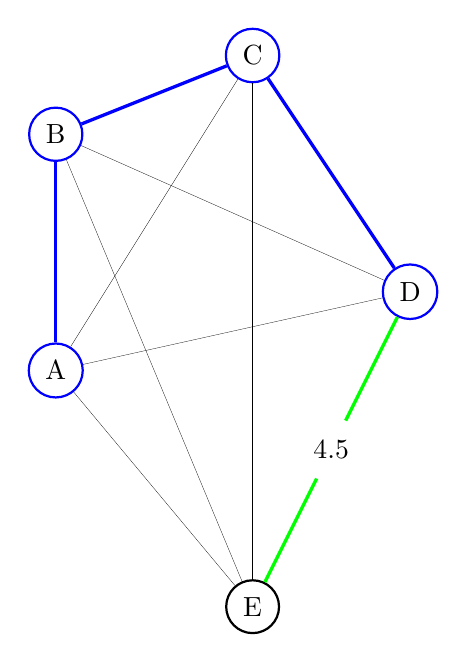
\begin{tikzpicture}
                \begin{scope}[every node/.style={circle,thick,draw}]
                    \node[draw=blue] (A) at (0,0) {A};
                    \node[draw=blue] (B) at (0,3) {B};
                    \node[draw=blue] (C) at (2.5,4) {C};
                    \node[draw=blue] (D) at (4.5,1) {D};
                    \node (E) at (2.5,-3) {E};
                \end{scope}

                \begin{scope}[every node/.style={fill=white,circle},
                            every edge/.style={draw=red,very thick}]
                    \path [-] (A) edge[draw=blue] (B);
                    \path [-] (B) edge[draw=blue] (C);
                    \path [-] (C) edge[draw=blue] (D);
                    \path [-] (E) edge[draw=black, ultra thin] (A);
                    \path [-] (A) edge[draw=black, ultra thin] (C);
                    \path [-] (A) edge[draw=black, ultra thin] (D);
                    \path [-] (B) edge[draw=black, ultra thin] (D);
                    \path [-] (B) edge[draw=black, ultra thin] (E);
                    \path [-] (C) edge[draw=black, ultra thin] (E);
                    \path [-] (D) edge[draw=green] node {$4.5$} (E);
                \end{scope}
            \end{tikzpicture}
        }
    \end{subfigure}$\Rightarrow$
    \begin{subfigure}[c]{0.2\textwidth}
        \centering
        \resizebox{\linewidth}{!}{
            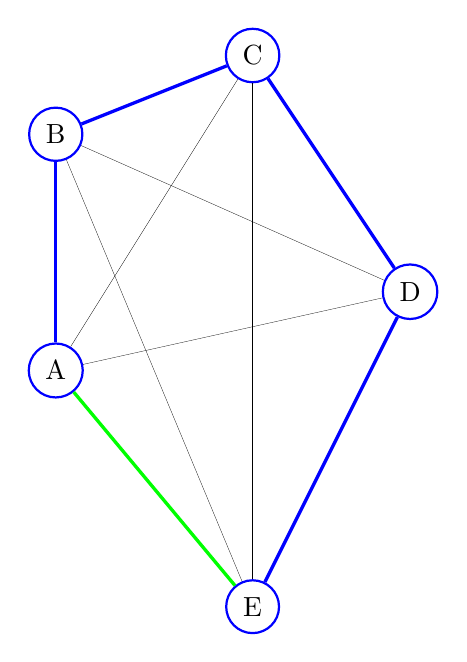
\begin{tikzpicture}
                \begin{scope}[every node/.style={circle,thick,draw}]
                    \node[draw=blue] (A) at (0,0) {A};
                    \node[draw=blue] (B) at (0,3) {B};
                    \node[draw=blue] (C) at (2.5,4) {C};
                    \node[draw=blue] (D) at (4.5,1) {D};
                    \node[draw=blue] (E) at (2.5,-3) {E};
                \end{scope}

                \begin{scope}[every node/.style={fill=white,circle},
                            every edge/.style={draw=red,very thick}]
                    \path [-] (A) edge[draw=blue] (B);
                    \path [-] (B) edge[draw=blue] (C);
                    \path [-] (C) edge[draw=blue] (D);
                    \path [-] (D) edge[draw=blue] (E);
                    \path [-] (E) edge[draw=green] (A);
                    \path [-] (A) edge[draw=black, ultra thin] (C);
                    \path [-] (A) edge[draw=black, ultra thin] (D);
                    \path [-] (B) edge[draw=black, ultra thin] (D);
                    \path [-] (B) edge[draw=black, ultra thin] (E);
                    \path [-] (C) edge[draw=black, ultra thin] (E);
                \end{scope}
            \end{tikzpicture}
        }
    \end{subfigure}$\Rightarrow$
    \begin{subfigure}[c]{0.2\textwidth}
        \centering
        \resizebox{\linewidth}{!}{
            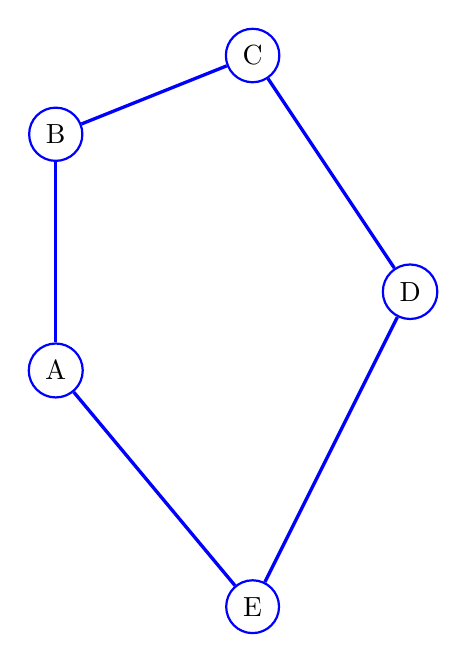
\begin{tikzpicture}
                \begin{scope}[every node/.style={circle,thick,draw}]
                    \node[draw=blue] (A) at (0,0) {A};
                    \node[draw=blue] (B) at (0,3) {B};
                    \node[draw=blue] (C) at (2.5,4) {C};
                    \node[draw=blue] (D) at (4.5,1) {D};
                    \node[draw=blue] (E) at (2.5,-3) {E};
                \end{scope}

                \begin{scope}[every node/.style={fill=white,circle},
                            every edge/.style={draw=red,very thick}]
                    \path [-] (A) edge[draw=blue] (B);
                    \path [-] (B) edge[draw=blue] (C);
                    \path [-] (C) edge[draw=blue] (D);
                    \path [-] (D) edge[draw=blue] (E);
                    \path [-] (E) edge[draw=blue] (A);
                \end{scope}
            \end{tikzpicture}
        }
    \end{subfigure}
    
\end{figure}

\FloatBarrier
\subsection{Pseudocode}
\begin{algorithm}[h]
    \caption{TSP greedy algorithm}

    \textbf{Input} starting node $s\in V$\\
    \textbf{Output} Hamiltonian cycle of V, cost of cycle\\
    \begin{algorithmic}

        \State $\mbox{cycle} \gets [s]$
        \State $\mbox{cost} \gets 0$
        
        \For{$i=0 \mbox{ to } n-2$}
            \State $\mbox{next}\gets\mbox{argmin}_v\{c(\mbox{cycle}[i],v) : v\in V - \mbox{cycle}\}$
            \State $\mbox{cost}\gets\mbox{cost}+c(cycle[i], next)$
            \State $\mbox{cycle}[i+1]\gets\mbox{next}$
        \EndFor
        \State $\mbox{cost}\gets\mbox{cost}+c(cycle[n-1],s)$\\\\
        \Return cycle, cost
    \end{algorithmic}
\end{algorithm}
\FloatBarrier

The solution found using the greedy algorithm is dependent on the starting node: a possible solution to this is to iterate through all possible starting nodes and keeping track of the best solution found so far.

\newpage

\subsection{Results analysis}
\begin{figure}[h]
    \centering
    \includegraphics*[width=.6\textwidth]{../solutions/1_600_greedy.jpg}
\end{figure}

The solutions found with the greedy algorithm are a good starting point, but sometimes the algorithm picks edges that cross a long distance, increasing the cost of the solution considerably.

This is caused by the fact that the greedy algorithm optimizes locally, without knowing whether that local choice is good or not in the long term: it might happen that after adding some edges to the cycle, the closest nodes are all already in the cycle, so the edge that will be considered may have a very large weight.

In the next section a tecnique to will fix this problem will explored.

\section{2-opt}

The 2-opt algorithm takes an existing cycle and tries to improve its cost by changing some of the edges that compose the cycle without breaking it.

The main idea behind the 2-opt algorithm is to find two edges that cross each other and fix them by removing the intersection:

\begin{figure}[h]

    \centering
    \begin{subfigure}[c]{.4\textwidth}
        \centering
        \resizebox{\linewidth}{!}{
            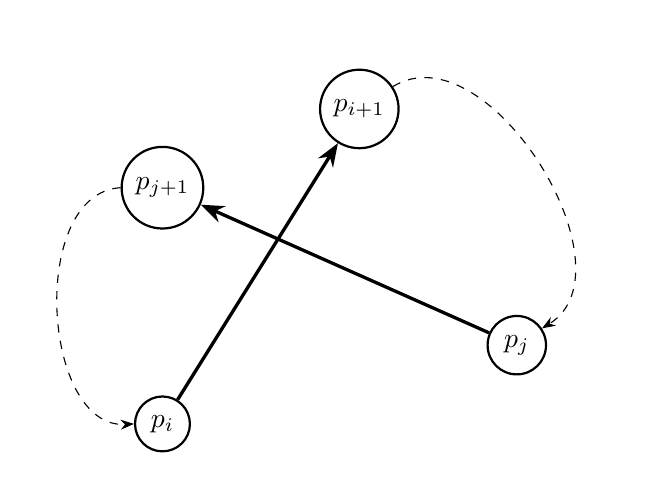
\begin{tikzpicture}
                \begin{scope}[every node/.style={circle,thick,draw}]
                    \node (I) at (0,0) {$p_i$};
                    \node (JJ) at (0,3) {$p_{j+1}$};
                    \node (II) at (2.5,4) {$p_{i+1}$};
                    \node (J) at (4.5,1) {$p_j$};
                \end{scope}

                \begin{scope}[>={Stealth[black]}, every node/.style={fill=white,circle},
                            every edge/.style={draw=red,very thick}]
                    \path[->] (I) edge[draw=black] (II);
                    \path[->] (J) edge[draw=black] (JJ);
                    \path[->] (JJ) edge[dashed, draw=black, thin, bend right=90] (I);
                    \path[->] (II) edge[dashed, draw=black, thin, bend left=90] (J);
                \end{scope}
            \end{tikzpicture}
        }
    \end{subfigure}
    \raisebox{-0.5\height}{$\Rightarrow$}
    \begin{subfigure}[c]{.4\textwidth}
        \centering
        \resizebox{\linewidth}{!}{
            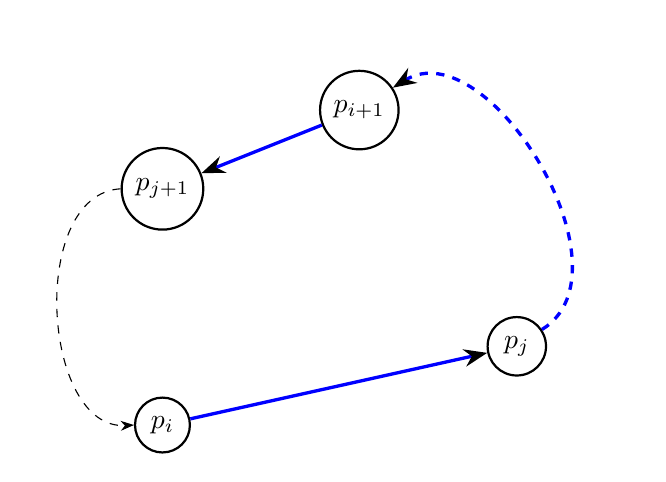
\begin{tikzpicture}
                \begin{scope}[every node/.style={circle,thick,draw}]
                    \node (I) at (0,0) {$p_i$};
                    \node (JJ) at (0,3) {$p_{j+1}$};
                    \node (II) at (2.5,4) {$p_{i+1}$};
                    \node (J) at (4.5,1) {$p_j$};
                \end{scope}

                \begin{scope}[>={Stealth[black]}, every node/.style={fill=white,circle},
                            every edge/.style={draw=red,very thick}]
                    \path[->] (I) edge[draw=blue] (J);
                    \path[->] (II) edge[draw=blue] (JJ);
                    %\path[-] (I) edge[dashed, draw=red, thin] (II);
                    %\path[-] (J) edge[dashed, draw=red, thin] (JJ);
                    \path[->] (JJ) edge[dashed, draw=black, thin, bend right=90] (I);
                    \path[->] (J) edge[dashed, draw=blue, bend right=90] (II);
                \end{scope}
            \end{tikzpicture}
        }
    \end{subfigure}
    \caption*{$p_i\coloneq\mbox{cycle}[i]$}

\end{figure}

This process is then repeated until no more edges that can lead to an improvement to the cost of the cycle can be found.

To find a pair of edges that can be changed to improve the cost it is sufficient to find a pair of nodes $p_i$, $p_j$ that satisfies the following inequality:

$$c_{p_i,p_{i+1}}+c_{p_j,p_{j+1}} > c_{p_i,p_{j}}+c_{p_{i+1},p_{j+1}}$$

Note that the cycle list is to be considered as a circular array: situations with indexes out of bounds or $i>j$ will not be treated in this paper since the fix is trivial.

If this inequality holds then swapping the edges $(p_i,p_j),\,(p_{i+1},p_{j+1})$ with $(p_i,p_{i+1}),$ $(p_{j},p_{j+1})$ will lower the cost of the cycle:

\begin{align*}
    \mbox{cost(new cycle)}&=\mbox{cost(old cycle)}-(c_{p_i,p_{i+1}}+c_{p_j,p_{j+1}})+(c_{p_i,p_{j}}+c_{p_{i+1},p_{j+1}})\\
    &\leq\mbox{cost(old cycle)}
\end{align*}

After finding the nodes $p_i$, $p_j$ the edges $(p_i, p_j)$ and $(p_{j+1}, p_{j+1})$ will take the place of the edges $(p_i, p_{i+1})$ and $(p_j, p_{j+1})$, reversing the route connecting $p_{i+1}$ to $p_{j}$.

Suppose the cycle is stored as a list of nodes ordered following the order of the nodes in the cycle, then this step can be done simply by reversing the list from the index $i+1$ to the index $j$:

$$[\ldots,p_i,\underline{p_{i+1},\ldots,p_j},p_{j+1},\ldots]\Rightarrow[\ldots,p_i,\underline{p_j,\ldots(\mbox{reversed})\ldots,p_{i+1}},p_{j+1},\ldots]$$

\subsection{Pseudocode}
\begin{algorithm}
    \caption{TSP 2-opt algorithm}

    \textbf{Input} Hamiltonian cycle of V, cost of cycle\\
    \textbf{Output} Hamiltonian cycle of V, cost of cycle\\
    \begin{algorithmic}

        \While{*a swap improving the cost exists*}
            \State $(i, j)\gets$ *find viable swap in the cycle*
            \State $\mbox{cost}\gets\mbox{cost}-(c(p_i,p_{i+1})+c(p_j,p_{j+1}))+(c(p_i,p_{j})+c(p_{i+1},p_{j+1}))$
            \State *reverse section of cycle between indices $i+1$ and $j$*
        \EndWhile\\\\

        \Return cycle, cost

    \end{algorithmic}
\end{algorithm}

\subsection{Swap policy}

In this paper two different ways of finding a swap have been compared:

\begin{enumerate}
    \item[-] returning the first swap found that improves the cost (referred as g2opt fs)
    \item[-] looking among all possible pair of edges and returning the swap that yields the largest cost improvement (the best swap, referred as g2opt bs)
\end{enumerate}

Using the performance profiler it is easy to see that the best swap policy finds solutions with an improvement of a 1\% factor with respect to the first swap policy:

\begin{figure}[h]
    \centering
    \includegraphics*[width=.6\textwidth]{perfprof_g2opt.png}
    \caption*{20 instances, size 600, Time limit: 120s}
\end{figure}

This is due to the fact that the first swap policy might get lost in improving the solution by a small amount by finding swaps in a region with an high concentration of nodes while the best swap policy aims to improve the edges with the highest weights.

This leads the best swap policy to fix immediately the worst edges, lowering right away the cost of the solution by a large amount.

\newpage

\subsection{A faster implementation}

The 2-opt algorithm is a good asset since it improves the solutions of a factor of 15\% with respect to the greedy solution, but it requires much more time (even in the multi thread version):
\begin{figure}[h]
    \centering
    \includegraphics*[width=.6\textwidth]{perfprof_g2opt_times.png}
    \caption*{20 instances, size 600, Time limit: 120s}
\end{figure}

As we can see, the 2-opt algorithm takes 15-20 times as much to reach these improvements: this slowdown gets worse with bigger problems seen the exponential time required to solve it.\\

The time needed by the 2-opt algorithm to fix the greedy solutions depends on the number of nodes, as stated before, but also on the quality of the solution that is being improved, so if we can somehow improve the solution before using the 2-opt algorithm, the time required to complete it will be much lower.\\

The idea is then to use a Divide and Conquer approach, applying the 2-opt algorithm to 2 subproblems and then applying it to the union of the 2 solutions to the subproblems.\\

\subsubsection{Pseudocode}
\begin{algorithm}
    \caption{TSP f2opt algorithm}

    \textbf{Input} Hamiltonian cycle of V, cost of cycle\\
    \textbf{Output} Hamiltonian cycle of V, cost of cycle\\
    \begin{algorithmic}

        \If{*reached max recursion depth*}
            \State (cycle, cost) $\gets$ *apply 2-opt to the cycle*\\
            $\quad\;\;$\Return cycle, cost
        \EndIf\\

        \While{*not reached max recursion depth*}
            \State (left, right) $\gets$ *split the cycle in two parts*
            \State (left, left\_cost) $\gets$ *apply the f2opt algorithm to the "left" part of the cycle*
            \State (right, right\_cost) $\gets$ *apply the f2opt algorithm to the "right" part of the cycle*
            \State (cycle, cost) $\gets$ *join (left, right) back into one cycle*
            \State (cycle, cost) $\gets$ *apply 2-opt to the cycle*
        \EndWhile\\\\

        \Return cycle, cost

    \end{algorithmic}
\end{algorithm}

The splitting procedure used consists in dividing the set of nodes in two parts based on their coordinates, so that in each of the two subsets obtained the nodes are close to each other.

The merging procedure consists just in gluing at random the two cycles together: trying some fancy ways of merging the two cycles would lead to a waste of computational resources since the 2-opt algorithm will be applied to the resulting cycle, probably re-arranging the edges made to glue the two cycles together.

This solution leads to a way faster algorithm thanks to having to apply the 2-opt algorithm on better solutions, bringing the slowdown down to 1.4. Another improvement that can be derived from this implementation is the fact that this version of 2-opt (called \textit{f2opt} from now on), is inherently parallel, letting us reach a slowdown of 1.2.

\begin{figure}[h]
    \centering
    \includegraphics*[width=.6\textwidth]{perfprof_f2opt_times.png}
    \caption*{20 instances, size 600, Time limit: 120s}
\end{figure}

\newpage 

\section{Comparison Greedy / 2-opt}

\begin{figure}[h]
    \centering
    \includegraphics*[width=.45\textwidth]{../plots/perfprof_heur_costs.png}
    \includegraphics*[width=.45\textwidth]{../plots/perfprof_heur_times.png}
    \caption*{20 instances, 600 nodes, time limit: 120s}
\end{figure}

The 2-opt algorithm manages to consistently improve the cost of the solutions of 15-20\% with respect to the solutions found by the greedy algorithm, while the f2opt alforithm reaches an improvement of 6-8\% whith a fraction of time needed by the basic 2-opt algorithm.

\begin{figure}[h]
    \centering
    \includegraphics*[width=.45\textwidth]{../solutions/1_600_greedy.jpg}
    \includegraphics*[width=.45\textwidth]{../solutions/1_600_g2opt.jpg}
    \caption*{20 instances, 600 nodes, time limit: 120s}
\end{figure}

As we can see, with the 2-opt algorithm, the solution is now free of crossing paths.

% Metaheuristics
\clearpage{\pagestyle{plain}\cleardoublepage}
\chapter{Metaheuristic}
A \textit{metaheuristic} is an abstact approach that can be applied to a range of problems, which can then be specialized. In our case, our metaheuristic algorithms use more than one heuristic in order to guide the search processs to efficiently explore the search space.

We explore two metaheuristic algorithm, which both unlock a greater search space compared to the aforementioned heuristic methods by allowing "bad moves" to escape a locally optimal solution.

\section{Tabu Search}
The \textit{tabu search} algorithm \cite{Glover1990} is based on the idea of allowing the 2-opt algorithm to perform swaps that still are the best ones, but not necessarily swaps that improve the cost of the solution. Once we find a local optima, the tabu search algorithm will keep searching, moving away from that locally optimal solution hoping to find a new one with a lower cost, whereas the 2-opt algorithm would stop.

If we allowed a bad move, at the next iteration the best move found by the 2-opt procedure would revert it, since that would be the only swap that lowers the cost. To prevent this, we need to keep track of those bad moves and prevent them from being reverted, marking them as \textit{tabu moves}, hence the name of the algorithm.

\subsection{Storing a tabu move}

A tabu move is intended as the worsening move that has been done in a previous round, and it basically consists on the 2 edges, or equivalently the 4 nodes, that were considered in the swap.

To store the tabu move we have more options on what to mark as a tabu move:

\begin{enumerate}
    \item one of the nodes (fix the two edges connected to that node)
    \item both nodes (fix all four edges in the swap)
    \item one or more edges
\end{enumerate}

Marking one or both nodes as tabu moves would restrict our area of search, since after a few tabu moves, lots of edges cannot be changed, so we opted to mark as a tabu move the two edges $(p_{i},p_{i+1})$ and $(p_{j}, p_{j+1})$.

\subsection{The tabu list}

The tabu list is intended as the list of tabu moves that 2-opt will need to consult to see whether a move is admitted or not. Once the tabu list is filled up, the oldest tabu move will be removed to let the one to be saved.

An important parameter of the tabu list is its size: a small size means that the algorithm is not very free to explore the search space, while a big size means that the algorithm will worsen the solution too much, possibly preventing it to ever find a better solution. This can also be intepreted as setting its memory: a small tabu list will forget earlier tabu moves, while a big tabu list will have a longer memory.

The size (or memory) of the tabu list will hereby be referred as the its \textit{tenure}. We built the tabu list as a fixed length array, where we stored each tabu move together with a counter which increases at each new tabu move. We used the counter to see if a move is still a tabu move or not: by comparing the current counter with the one stored along the move, we can check how many iterations has passed and if more iterations than the tenure has occurred, that moves is no longer a tabu move.

We tried out two ways of checking the tenure:

\begin{enumerate}
    \item \textit{static approach}: a move in the list is no longer a tabu move if
    $$\text{counter}-\text{counter(move)} < \text{tenure}$$
    where $\text{counter(move)}$ is the counter stored along the move in the tabu list.
    \item \textit{dynamic approach}: a move in the list is no longer a tabu move if
    $$\text{counter}-\text{counter(move)} < f(\text{tenure}, \text{counter})$$
    where $f(\text{tenure},\text{counter})\coloneq A\cdot\sin(\text{counter}\cdot B) + \text{tenure}$, and $A$, $B$ are parameters specified by the user (A will be referred as variable\_tenure).
\end{enumerate}

The dinamic approach performs better for a few reasons:

\begin{enumerate}
    \item it lowers the risk of remaining stuck for many iterations: when we reach a local optimum, with the dynamic approach the algorithm will start to forget some moves in a few iterations and will escape from that situation;
    \item it allows for a more dynamic exploration of the search space: the dynamic approach allows the algorithm to "forget" something to look for a better solution in the search space, but then remember it later if that leads to nothing.
\end{enumerate}

\subsection{Pseudocode}

\begin{algorithm}
    \caption{TSP tabu search algorithm}
    
    \textbf{Input} starting node $s\in V$\\
    \textbf{Output} Hamiltonian cycle of V, cost of cycle\\
    \begin{algorithmic}
        
        \State (cycle, cost) $\gets$ *result of greedy algorithm on $s$ and $V$*\\

        \While{*time limit not exceeded*}
            \State $(i, j)\gets$ *swap to be applied on cycle (checking the tabu list)*
            \If{*swap (i,j) leads to a worse position*}
                \State *add $(i,j)$ to tabu list*
            \EndIf
            \State *update cost*
            \State *reverse section of cycle between indices $i+1$ and $j$*

        \EndWhile\\\\

        \Return cycle, cost
    \end{algorithmic}
\end{algorithm}

Where the $\mbox{find\_tabu\_swap()}$ method returns the best swap (allowing for bad moves) after checking the tabu list.

\subsection{Results analysis}

\begin{figure}[h]
    \centering
    \includegraphics*[width=.6\textwidth]{../plots/perfprof_tabu_costs.png}
    \caption*{20 instances, 600 nodes, time limit: 120s}
\end{figure}
\FloatBarrier

This plot reports various executions of the tabu algorithm with different parameters: the first two use a tenure of 1/10 and 1/5 of the number of nodes while using the static tenure approach; the last two use the dynamic approach insthead, whith a variable\_tenure of 1/10 and 1/5 of the number of nodes.

As we expected, the dynamic approach yields slightly better results than the static approach. It is important to point out that the latter generates worse solutions than the 2-opt algorithm: this is due to the fact that the 2-opt algorithm looks among all possible greedy solutions based on the starting node, while the tabu algorithm only uses one starting point to explore the search space (or a fixed amount if using multithreading).\\

We can see how the dynamic approach manages to surpass this limitation and improve the solutions with respect to the 2-opt algorithm.

\section{Variable Neighborhood Search (VNS)}

For the tabu algorithm to work, a list of moves must be stored as tabu moves: how many moves to store? Which one works better: a static or a dynamic tenure? And in the latter, how much should the tenure vary? This set of hyperparameters should be set with procedures that are unaffordable for the scope of this thesis. We may also run into overfitting.

A metaheuristic method that does not require hyperparameters is the \textit{Variable Neighborhood Search (VNS)} \cite{Hansen2019}, which approaches the same base idea of tabu search in a different way. Once we are in a local minimum, if we make a 2-opt swap (as we do with the tabu search algorithm), we must save that move as a tabu move, since the next 2-opt swap will revert it. The VNS approach is to make a swap that requires more than two edges to be swapped (entering the family of k-opt), in our case a 3-opt swap. Once a 3-opt swap is performed, it is impossible for a 2-opt swap to reverse that change, since it should change 3 edges and is allowed to change only 2 of them.

In some scenarios one 3-opt swap is enough to escape the local minimum, but in other it is not and more swaps are needed, thus creating a hyperparameter. To prevent this, we used multithreading to perform different numbers of 3-opt swaps on a local minimum, then use the 2-opt algorithm to lower the cost, and choose the best among the solutions found.

Another approach that can be explored in the future is using multithreading to keep the $k$ best choices among the solutions found and keep exploring them in parallel, with special attention to keep the list of parallel runs under control, avoiding exponential growth.

\newpage

\subsection{Pseudocode}

\begin{algorithm}
    \caption{TSP VNS algorithm}
    
    \textbf{Input} starting node $s\in V$\\
    \textbf{Output} Hamiltonian cycle of V, cost of cycle\\
    \begin{algorithmic}
        
        \State (cycle, cost) $\gets$ *result of greedy algorithm on $s$ and $V$*\\

        \While{*time limit not exceeded*}\\

            \State (cycle, cost) $\gets$ *apply random kicks to the cycle*
            \State (cycle, cost) $\gets$ *apply 2-opt to the cycle*\\

        \EndWhile\\\\

        \Return cycle, cost
    \end{algorithmic}
\end{algorithm}

The kicks we applied are 3-opt swaps using the following schema:

\begin{figure}[h]

    \centering
    \begin{subfigure}[c]{.4\textwidth}
        \centering
        \resizebox{\linewidth}{!}{
            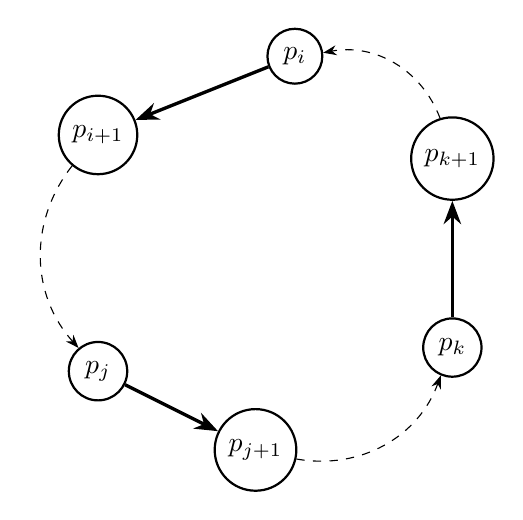
\begin{tikzpicture}
                \begin{scope}[every node/.style={circle,thick,draw}]
                    \node (I) at (2.5,4) {$p_i$};
                    \node (II) at (0,3) {$p_{i+1}$};
                    \node (J) at (0,0) {$p_j$};
                    \node (JJ) at (2,-1) {$p_{j+1}$};
                    \node (K) at (4.5,0.3) {$p_k$};
                    \node (KK) at (4.5,2.7) {$p_{k+1}$};
                \end{scope}

                \begin{scope}[>={Stealth[black]}, every node/.style={fill=white,circle},
                            every edge/.style={draw=red,very thick}]
                    \path[->] (I) edge[draw=black] (II);
                    \path[->] (J) edge[draw=black] (JJ);
                    \path[->] (K) edge[draw=black] (KK);
                    \path[->] (II) edge[dashed, draw=black, thin, bend right=40] (J);
                    \path[->] (JJ) edge[dashed, draw=black, thin, bend right=40] (K);
                    \path[->] (KK) edge[dashed, draw=black, thin, bend right=40] (I);
                \end{scope}
            \end{tikzpicture}
        }
    \end{subfigure}
    \raisebox{-0.5\height}{$\Rightarrow$}
    \begin{subfigure}[c]{.4\textwidth}
        \centering
        \resizebox{\linewidth}{!}{
            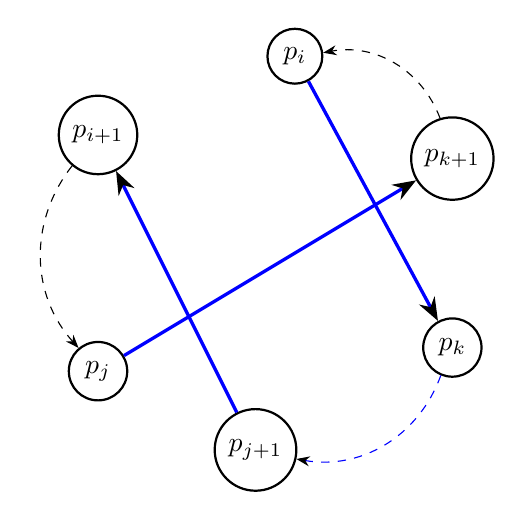
\begin{tikzpicture}
                \begin{scope}[every node/.style={circle,thick,draw}]
                    \node (I) at (2.5,4) {$p_i$};
                    \node (II) at (0,3) {$p_{i+1}$};
                    \node (J) at (0,0) {$p_j$};
                    \node (JJ) at (2,-1) {$p_{j+1}$};
                    \node (K) at (4.5,0.3) {$p_k$};
                    \node (KK) at (4.5,2.7) {$p_{k+1}$};
                \end{scope}

                \begin{scope}[>={Stealth[black]}, every node/.style={fill=white,circle},
                            every edge/.style={draw=red,very thick}]
                    \path[->] (I) edge[draw=blue] (K);
                    \path[->] (JJ) edge[draw=blue] (II);
                    \path[->] (J) edge[draw=blue] (KK);
                    \path[->] (II) edge[dashed, draw=black, thin, bend right=40] (J);
                    \path[->] (K) edge[dashed, draw=blue, thin, bend left=40] (JJ);
                    \path[->] (KK) edge[dashed, draw=black, thin, bend right=40] (I);
                \end{scope}
            \end{tikzpicture}
        }
    \end{subfigure}
    \caption*{$p_i\coloneq\mbox{cycle}[i]$}

\end{figure}

Note that, if we follow this schema, we need to reverse the cycle between $p_{j+1}$ and $p_k$.

\newpage

\section{Comparison Tabu Search / VNS}

\FloatBarrier
\begin{figure}[h]
    \centering
    \includegraphics*[width=.6\textwidth]{../plots/perfprof_met_costs_result.png}
    \caption*{20 instances, 600 nodes, time limit: 120s}
\end{figure}

As we can see, the VNS algorithm has consistently better performances than the tabu search algorith, up to a 3\% improvement: this might be due to the fact that the tabu search algorithm requires a finer parameter tuning, while the VNS algorithm does not need any.

% Exact methods
\clearpage{\pagestyle{plain}\cleardoublepage}
\chapter{Exact methods}
The exact algorithms for the TSP algorithm described in this section are all based on \textit{CPLEX}, which uses a proprietary implementation of the \textit{branch \& bound (B\&B)} method to return a solution to the input model. Most of the times, we can expect an "optimal" solution with an integrality gap close to zero. However, since it is computationally infeasible to add every possible SEC to the model, CPLEX will return a solution which is feasible for its internal model but infeasible for our original TSP problem. Thus, we use various techniques to find a good solution for the TSP problem using CPLEX.

\section{Benders' loop}
A simple approach to use SECs without computing all of them is the \textit{Benders' loop} technique. We start with a model with no SECs. Given the solution returned by CPLEX, we identify its various connected components and compute the SECs on those components alone. We repeat the procedure with the new model until we get a solution with only one connected component or we exceed the timelimit.

This method is guaranteed to reach a feasible solution for the TSP problem if the timelimit is not exceeded, but this will happen only at the final iteration: if the time runs out before we find such feasible solution, we will have an infeasible one with multiple connected components. Moreover, it does not always improve the lower bound for the final solution, since the number of connected components of the solutions found throughout the algorithm's execution is not always decreasing.

\FloatBarrier
\subsection{Pseudocode}
\begin{algorithm}[h]
    \caption{Benders' loop}
    \hspace*{\algorithmicindent} \textbf{Input} undirected complete graph $G=(V,E)$, cost function $c:V\rightarrow\mathbb{R}$\\
    \hspace*{\algorithmicindent} \textbf{Output} List of $n\coloneq|V|$ nodes forming an Hamiltonian cycle, cost of the cycle
    \begin{algorithmic}

        \State build CPLEX model from $G$ with objective function and degree constraints
        \While{timelimit not exceeded}
        \State $x^* \leftarrow$ solution of CPLEX model
        \State determine connected components of $x^*$
        \If{$x^*$ has only connected component}
        \Return $x^*$
        \EndIf
        \ForEach{connected component $S\subset V$ in $x^*$}
        \State add SEC to model: $\sum_{e\in\delta(S)}x_e\leq|S|-1$
        \EndFor
        \EndWhile

    \end{algorithmic}
\end{algorithm}
\FloatBarrier

\section{Patching heuristic}
The major flaw of this method is returning a feasible solution only at the very last iteration. A possible solution to this issue is the implementation of a \textit{patching} heuristic. Given the CPLEX solution at any iteration, we patch together the various connected components to provide a feasible solution even if the timelimit is exceeded before getting a solution with a single component.

Two components $k1\neq k2\subset V$ are patched by replacing two edges $(p_i, p_{i+1})\in k1$ and $(p_j, p_{j+1})\in k2$ with the pair of edges of minimal cost between $(p_i,p_j), (p_{i+1},p_{j+1})$ and $(p_i,p_{j+1}),(p_j, p_{i+1})$. We iterate through all combinations of $k1,k2$ to find the swap with the lowest increase in cost. Once we find the swap, we perform it and repeat the process until we are left with only one connected component.

This procedure may introduce some crossing edges into $x^*$. Thus, we apply the 2opt algorithm after this procedure to remove them.

\newpage
\subsection{Pseudocode}
\begin{algorithm}[h]
    \caption{Patching heuristic Benders' loop}
    \hspace*{\algorithmicindent} \textbf{Input} solution $x^*$ returned by CPLEX with $ncomp$ connected components\\
    \hspace*{\algorithmicindent} \textbf{Output} $x^*$ with 1 connected component
    \begin{algorithmic}

        \While{$ncomp\neq1$}
        \State $best\_k1\leftarrow0, best\_k2\leftarrow0, best\_delta\leftarrow-\infty$;
        \For{$k1\leftarrow0$ to $ncomp-1$, $k2\leftarrow k1+1$ to $ncomp-1$}
        \ForEach{$(p_i,p_{i+1})\in x^*$ with $p_i,p_{i+1}\in k1$}
        \ForEach{$(p_j,p_{j+1})\in x^*$ with $p_j,p_{j+1}\in k2$}
        \State $delta\_N\leftarrow$ change in cost of solution produced by replacing
        \State $(p_i,p_{i+1}), (p_j,p_{j+1})$ with $(p_i,p_{j+1}), (p_j,p_{i+1})$ in $x^*$;
        \State $delta\_R\leftarrow$ change in cost of solution produced by replacing
        \State $(p_i,p_{i+1}), (p_j,p_{j+1})$ with $(p_i,p_j), (p_{j+1},p_{i+1})$ in $x^*$;
        \State $delta\leftarrow\max\{delta\_N,delta\_R\};$
        \If{$delta>best\_delta$}
        \State $best\_delta \leftarrow delta$;
        \EndIf
        \EndFor
        \EndFor
        \EndFor

        \State patch components $best\_k1,best\_k2$ applying transformation with change in cost
        \State $delta$;
        \State cost of $x^* \leftarrow$ cost - $best\_delta$;
        \State $ncomp \leftarrow ncomp-1$;
        \EndWhile
    \end{algorithmic}
    
\end{algorithm}

\subsection{Algorithm comparison}

We compared the results obtained by Benders' loop both with and without the patching heuristic. Within this timeframe the algorithms produced solutions with the same costs but took different amounts of time.

\FloatBarrier
\begin{figure}[h]
    \centering
    \includegraphics*[width=.6\textwidth]{../plots/perfprof_benders_times.png}
    \caption*{20 instances, 300 nodes, time limit: 360s}
\end{figure}
\FloatBarrier

The patching heuristic allowed the algorithm to reach a feasible solution in less time. This is in line with the nature of Benders' loop: the base version of the algorithm produces a feasible solution only at the very last iteration, an issue that can be avoided by patching the components after every iteration.

% Matheuristics methods
\clearpage{\pagestyle{plain}\cleardoublepage}
\chapter{Matheuristics}
Up to this point we have explored two different approaches to solving the TSP problem that can be considered the extremes of a scale. On one hand we have several heuristic algorithms that can quickly solve instances with little guarantee of finding an optimal solution; on the other hand we have exact algorithms based on cplex, which can find optimal solutions for small instances.

As a compromise between the two, we implemented a series of hybrid methods called \textit{matheuristics} \cite{Fischetti2016}. These methods take a closed-box MIP solver, that is guaranteed to find an optimal solution to the model they receive in input, and we use it as a heuristic; this is achieved by giving as input a restricted version of the original model, from which an arbitrary set of feasible solutions has been excluded. In this way, we still exploit the power of the MIP solver, while restricting the space of possible solutions, thus reducing the required time to solve the model.

\section{Diving}

This matheuristic is based on iteratively solving the TSP model and restricting it by taking the best solution found up to a certain iteration and \textit{hard fixing} some of its edges, using a heuristic solution as the starting incumbent. These edges are called \textit{'yes' edges} and they are fixed by setting the values of their respective variables in the model to 1. This method is called \textit{diving} because fixing a series of variables is analogous to reaching a certain depth of the branch \& bound tree in a single iteration.

There are several possible approaches to decide how many and which edges to fix. In this paper we choose them in a completely random way. While it is the simplest possible approach, it has the advantage of having a very small probability of getting stuck on a certain neighborhood of solutions.

\newpage

\subsection{Pseudocode}
\begin{algorithm}[h]
    \caption{Diving matheuristic algorithm}
    \textbf{Input} $pfix$ edge fixing probability\\
    \textbf{Output} Hamiltonian cycle of G, cost of cycle\\
    \begin{algorithmic}

        \State $x^H \gets$ *heuristic solution of TSP on G*
        \State *build CPLEX model from $G$ with objective function and degree constraints*\\
        \While{*time limit not exceeded*}
        \State $\tilde{E} \gets$ *subset of $E$ with $|V|*pfix$ edges of $x^H$ chosen at random with probability $pfix$*
        \State *fix every $x_e^H\in\tilde{E}$ to $1$ in model*\\
        \State *$x^*\gets$ solution returned by CPLEX for input model with fixed edges*
        \If{$\text{cost}(x^*)\leq \text{cost}(x^H)$}
        \State $x^H\gets x^*$
        \EndIf\\
        \State *unfix every $x_e^H\in\tilde{E}$ in model*
        \EndWhile

    \end{algorithmic}
\end{algorithm}
\FloatBarrier

\subsection{Hyperparameter tuning}

$pfix$ is a hyperparameter of the algorithm, thus we tested different values for it.

\begin{figure}[h]
    \centering
    \includegraphics*[width=.6\textwidth]{../code/plots/perfprof_hard_costs.png}
    \caption*{20 instances, 1000 nodes, time limit: 120s}
\end{figure}
\FloatBarrier

The diving algorithm yields worse solutions than our best CPLEX solver. As we saw, the major performance boost we had when testing the different CPLEX settings came from patching and posting solutions inside the callbacks. Since by patching we might generate solutions which would be rejected by the model with the fixed variables, much of this work is performed in vain; this might be the cause of this performance drop.

\section{Local Branching}

In the diving algorithm, we decided both how many and which variables to fix in the mathematical problem before using the CPLEX solver. In the \textit{local branching} algorithm \cite{Fischetti2003}, instead, we choose only how many variables we want to fix, leaving to the TSP solver the responsibility of choosing which ones to fix. This is expressed in the model by adding an additional constraint.

Given $x^H$ the current incumbent, we define the \textit{local branching constraint} as:
$$\sum_{e:x^H_e=1}x_e\geq n-k$$
The left-hand sum is the number of variables we want the TSP solver to keep from $x^H$, while $k$ is the number of variables we want the TSP solver to fix. By setting the direction of the constraint as $\geq$, the solver explores a neighborhood of different solutions that can be reached by changing $n-k$ variables (looking for the best k-opt swap to apply).

This constraint is not guaranteed to be valid for the set of feasible solution, because it might cut out the optimal solution; however, it allows us to greatly reduce the integrality gap.

\FloatBarrier
\subsection{Pseudocode}
\begin{algorithm}[h]
    \caption{Local branching matheuristic algorithm (v1)}
    \textbf{Input} integer $k_{\text{init}}$\\
    \textbf{Output} Hamiltonian cycle of G, cost of cycle\\
    \begin{algorithmic}

        \State $x^H \gets$ *heuristic solution of TSP on G*
        \State *build CPLEX model from $G$ with objective function and degree constraints*
        \State $k\gets k_{\text{init}}$
        \While{*time limit not exceeded*}
        \State *add constraint local branching constraint $\sum_{e:x_e^H=1}x_e\geq n-k$*
        \State $x^*\gets$ *solution returned by CPLEX for input model with local branching constraint*
        \If{$\text{cost}(x^*)\leq \text{cost}(x^H)$}
        \State $x^H\gets x^*$
        \EndIf
        \If{*$x^H$ has not been improved for 5 iterations*}
        \State $k\gets k+10$
        \EndIf
        \State *save improvements*
        \State *remove local branching constraint*
        \EndWhile\\\\

        \Return $x^H$, $\text{cost}(x^H)$

    \end{algorithmic}
\end{algorithm}
\FloatBarrier

\subsection{Hyperparameter tuning}

In this algorithm, $k_{\text{init}}$ is the hyperparameter.

\begin{figure}[h]
    \centering
    \includegraphics*[width=.6\textwidth]{../code/plots/perfprof_lbv1_costs.png}
    \caption*{20 instances, 1000 nodes, time limit: 120s}
\end{figure}

Similarly to the diving algorithm, the gap between the costs found by our best CPLEX solver and the local branching algorithm is smaller than 10\%. We can also see an improvement for greater starting values of $k$.

\subsection{A more dynamic approach}
The choice of $k$ helps us reducing the integrality gap, so we might want to change this value dynamically based on the results of each iteration of the local branching algorithm.

As we can see, with this approach the algorithm manages to move through the search space more smoothly, improving its performances of a 6-8\% factor, beating our best CPLEX setting.

\begin{figure}[h]
    \centering
    \includegraphics*[width=.6\textwidth]{../code/plots/perfprof_lb_costs.png}
    \caption*{20 instances, 1000 nodes, time limit: 120s}
\end{figure}

\begin{algorithm}[h]
    \caption{Local branching matheuristic algorithm (v2)}
    \textbf{Input} integer $k_{\text{init}} = 100$\\
    \textbf{Output} Hamiltonian cycle of G, cost of cycle\\
    \begin{algorithmic}

        \State $x^H \gets$ *heuristic solution of TSP on G*
        \State *build CPLEX model from $G$ with objective function and degree constraints*
        \State $k\gets k_{\text{init}}$

        \While{*time limit not exceeded*}

            \If{*this is a new iteration*}
                \State *add constraint local branching constraint $\sum_{e:x_e^H=1}x_e\geq n-k$*
                \State *add the best solution found so far as a warm start*
            \EndIf

            \State $x^*\gets$ *solution returned by CPLEX for input model with local branching constraint*

            \If{*CPLEX exited for time limit and no visible improvement*}

                \If{*more than 3 repetitions*}
                    \State $k\gets k+10$
                    \State *finish this iteration*
                \Else
                    \State *repeat this iteration without changing CPLEX model*
                \EndIf
            \Else
                \If{*CPLEX found optimal solution for this model*}
                    \State $k\gets k-10$
                \EndIf
            \EndIf

            \State *save improvements*
            \State *remove local branching constraint*

        \EndWhile\\\\

        \Return $x^H$, $\text{cost}(x^H)$

    \end{algorithmic}
\end{algorithm}

\newpage

\subsection{Considering multiple solutions}

The idea behind local branching is to limit the search space using a solution that we know is feasible, but not optimal. The constraint we add to the model ensures that we only fix how many edges we want to take from the solution found in the past iteration. If we want to consider more than one past solution, we can use this variation of the constraint:
$$\sum_{e\in E}\mbox{count}(e)\cdot x_e\geq n-k$$
where count($e$) is the number of times edge $e$ has been considered in past solutions. Note that if we consider just the solution from the last iteration of local branching, count($e$)$\in\{0,1\} \ \forall e\in E$, which leads to the first version of the constraint.

With this constraint we give more importance to edges that have been considered "optimal" in more than one solution. We follow the hypotesis that edges that are found more times are more likely to be in the optimal solution.

The mathematical meaning of the constraint is changed: in the normal local branching, $k$ is the exact number of edges that CPLEX can change, while in this constraint this claim does not hold. The left-hand side of the constraint now gives more importance to edges whose count is greater than 1; if CPLEX chooses to fix an edge with an high count, it has a bigger search space, since count($e$) will bring the lower bound $n-k$ closer, hence it now has more freedom.

To sum up, with this constraint CPLEX will still search the best k-opt swap around the suggested solution, but it will also try solutions with more swaps around solutions whose edges have been already considered in other iterations of the local branching.

\subsection{Results analysis}

This new constraint is not optimal: if the number of solutions considered start to increase indefinitely the left-hand side of the constraint will reach large values, so large that the meaning of the degrees of freedom that we give to CPLEX, $k$, will start to vanish.

In our implementation this is not a problem since we give each iteration of local branching 1/10 of the total time limit, so at most $\text{count}(e)\leq10$. Moreover, with the v2 version of the algorithm illustrated in section 6.2.3 we almost never reach such a high count.

To avoid this problem, we made two different versions of this local branching: one that considers each of the past solutions found, and one which considers only a fixed number of recent past solutions.

\begin{figure}[h]
    \centering
    \includegraphics*[width=.6\textwidth]{../code/plots/perfprof_lbv2_costs.png}
    \caption*{20 instances, 1000 nodes, time limit: 120s}
\end{figure}

Here we can see that using the new constraint gives slightly better solutions than the original one and that limiting the number of past solutions considered in the constraint does not make a difference, as previously explained.

\section{Comparison diving / local branching}

\begin{figure}[h]
    \centering
    \includegraphics*[width=.6\textwidth]{../code/plots/perfprof_mat_costs.png}
    \caption*{20 instances, 1000 nodes, time limit: 120s}
\end{figure}

Beating our best CPLEX solver was hard given the range of optimization techniques we used, but in the end we managed to find a matheuristic method which can help us with problems which are too big for CPLEX to handle by itself.

% Conclusions
\clearpage{\pagestyle{plain}\cleardoublepage}
\chapter{Conclusions}
To sum up the performances of the algorithms proposed, this performance profile compares the best algorithms among metaheuristic, exact and matheuristic approaches:

\begin{figure}[h]
    \centering
    \includegraphics*[width=.6\textwidth]{../plots/perfprof_conclusions.png}
    \caption*{20 instances, 1000 nodes, time limit: 120s}
\end{figure}

As we can see, our implementation of the vns algorithm manages to compete with our best CPLEX solver: this is thanks to the speed of the f2opt algorithm which is used to find the first local minimum, since the 2-opt algorithm requires too much time with instances of such size.

The best algorithm for large instances still remains the local branching, which manages to navigate the search space efficiently thanks to our multiple solutions approach to the construction of the constraint.

\section{Future works}
The algorithms proposed are far from optimal and could use some improvements.

Currently the f2opt algorithm merges the sub sub-problems randomly, but an approach similar to the patching seen in section 5.2 could be applied.

The tabu algorithm uses multithreading by performing multiple searches from different starting point at the same time, while the vns algorithm uses it to choose the best number of kicks to do: finding a better way to use multithreading in our tabu search algorithm might close the gap between those two metaheuristic methods.

We could invest some time looking for better patching algorithms for our fractionary solutions, so that in the relaxation callback we can post solutions with an higher quality, lowering the upper bound inside CPLEX.

One last improvement we could make is to further explore the idea of using multiple solutions inside the local branching algorithm: we might use different statistics rather than the number of times an edge has been selected and we might find a better right-hand side to our constraint, so that the degrees of freedom given by that constraint is more controlled.

\afterpage{\blankpage}
    
% Bibliography
%\clearpage{\pagestyle{plain}\cleardoublepage}
%\chapter{Bibliography}
%\input{chapters/bibliography}

\printbibliography

\end{document}